\documentclass[a4paper,10pt]{article}

\usepackage[inner=3cm,top=3cm,outer=3cm,bottom=3cm]{geometry}
\usepackage[parfill]{parskip} % line skip between paragraphs instead of indents
\usepackage{fancyhdr}
\usepackage{fancyvrb}
\usepackage{graphicx}
\usepackage{xcolor}
\usepackage{color, colortbl}
\usepackage{setspace} % dynamic line spacing
\usepackage{float} % picture placing
\usepackage{caption}
\usepackage{verbatim} % insert files verbatim
\usepackage{pdfpages} % import raw pdf
\usepackage[toc,page]{appendix}
\usepackage[labelformat=empty]{caption} % picture captions
\ifxetex
  % babel for xetex
  \usepackage{fontspec}
  \usepackage{polyglossia}
  \setdefaultlanguage{swedish}
	% i xetex behövs inga fulhack för åäö
\else
	% åäö-hax för icke-xelatex
  \usepackage[swedish]{babel}
	\usepackage[utf8]{inputenc}
  \usepackage[T1]{fontenc}
\fi
\usepackage[style=authoryear,backend=biber]{biblatex} % harvard citing, modern backend
\usepackage{csquotes} % language aware quoting
\usepackage{hyperref} % automatic pdf bookmarks and hyperlinks, must be loaded last

\bibliography{reference} % link to bibliography bib file

% Header and footer
\pagestyle{fancy}\headheight 13pt
\fancyfoot{} % reset footer format
\fancyfoot[LE,RO]{\thepage}
\renewcommand{\headrulewidth}{0pt}
\renewcommand{\footrulewidth}{0pt}

% configuration
\def\thetitle{URD-2}
\def\groupname{The Meta Family}
\def\groupmembers{Daniel Bergström \\ Paulina Hensman \\ Marcus Hertz \\ Simon Karlsson \\ David Masko \\ Marcus Nordberg \\ André Nyström \\ William Perkola \\ Axel Riese \\ Kerry Zhang}
\def\version{Version 2.0}
\def\thedate{\today}
\renewcommand{\arraystretch}{1.2} % spacious tables

%----------------------------------------------------------------------------------------
%	TITLE PAGE
%----------------------------------------------------------------------------------------

\newcommand*{\titleGM}{\begingroup % Create the command for including the title page in the document
\hbox{ % Horizontal box
\hspace*{0.1\textwidth} % Whitespace to the left of the title page
\parbox[b]{0.75\textwidth}{ % Paragraph box which restricts text to less than the width of the page

{\noindent\Huge\bfseries \thetitle \\[0.5\baselineskip] \groupname}\\[2\baselineskip] % Title

{\large \version \\[\baselineskip] den \thedate}\\[2\baselineskip] 

\begin{doublespace}
{\Large \groupmembers} % Author name
\end{doublespace}

}}
\endgroup}


% pdf metadata
\hypersetup{pdfinfo={
Title={URD-2},
Author={The Meta Family}
}}

\begin{document}

% title page
\thispagestyle{empty}
\titleGM
\clearpage

% empty/icon page
\thispagestyle{empty}

\includepdf{metafam.pdf}
\clearpage 

% abstract
\thispagestyle{empty}
\section*{Sammanfattning} %unnumbered
Denna projektplaneringsrapport behandlar implementeringen av en SDK (Software development kit) till Android för applikationstestning.
\clearpage

% table of contents
% generated automatically
% from \section commands
\thispagestyle{empty}
\tableofcontents % babel/polyglossia fixar språket
\clearpage

% document change record
\setcounter{page}{1}
\section*{Versionshistorik}
% add to table of contents, but no numbering
\addcontentsline{toc}{section}{Versionshistorik}
\subsection*{0.1}
Första utkast. Varje underrubrik utom abstract är färdigskriven men texten är ej korrekturläst.

\subsection*{0.2}
Rapporten har uppdaterats med ett abstract.

\subsection*{1.0}
Alla delar är på plats. Gruppen anser att rapporten är färdig för inlämning.

\subsection*{1.1}
Mindre korrigering av källa.

\clearpage

\begin{flushleft} % left align
\section{Introduktion}

\subsection{Syfte}

Syftet med dokumentet är att ge en överblick av SuperRecorder-projektet, både för projektgruppen och kunden The Beta Family. I dokumentet finns all information om vad som ingår i projektet och alla eventuella svårigheter som hittats. Det går att läsa om hur de olika delarna kommer implementeras och hur de hänger ihop med varandra. Dokumentet ska ses som en sammanställning av kundens krav, våra utredningar av möjliga lösningar och våra slutliga lösningsförslag. Projektgruppen kommer efter bästa förmåga genomföra lösningarna som det står skrivet i dokumentet, men ger inga garantier på att slutresultatet helt stämmer överens med våra förslag.

Den kravspecifikation som definieras under punkt 2.2 och punkt 3 anses bindande tillsvidare. Dokumentets övriga punkter reflekterar informella överenskommelser mellan gruppen och kunden.

\subsection{Produktens omfång}
Produkten är ett SDK för Android som riktar sig till applikationsutvecklare. SDK:t möjliggör dokumentering av användartester. Testaren kan välja att dokumentera skärmen med rörelsehändelser, röst och front-kamera.

\subsection{Begreppsdefinitioner}

\emph{Applikation} Körbart program i smartphones, förkortas ibland till ``app''.

\emph{Applikationsutvecklare} Person som utvecklar applikationer, förkortas  ibland till ``apputvecklare''.

\emph{Bitmap} Grupp lagringsformat för digitala biler där ingen data går förlorad. Lämpad för exempelvis skärmdumpar.

\emph{FPS} Frames per seconds, bilder per sekund. Vanligt mått på bildhastighet i video.

\emph{GUI} Graphical User Interface är det gränsnitt som en användare av ett program ser och interagerar med.

\emph{iOS} Namnet på det operativsystem som används på Apples smartphones.

\emph{Laravel} Ett ramverk byggt främst i PHP för att förenkla utvecklandet av skalbara webbapplikationer\parencite{laravel}.

\emph{PHP} PHP: Hypertext Preprocessor (\textit{rekursiv akronym}) är ett programmeringsspråk som körs på webbservern för att hantera dynamiskt innehåll på webbplatser.

\emph{Protokoll} Samordnad överenskommelse mellan utvecklare av separata system om hur data skall skickas för att möjliggöra korrekt mottagande av data.

\emph{SDK} Software Development Kit är en mängd verktyg som gör det möjligt för en utvecklare att bygga en viss mjukvara. Det kan röra sig om allt från ett enskilt bibliotek som tillhandahåller en mängd funktioner till en komplett utvecklingsmiljö.

\emph{TBF} The Beta Family, vår projektbeställare.

\emph{Zurb} Ett ramverk byggt i HTML, CSS och JavaScript för att underlätta front-end-utveckling hos webbapplikationer\parencite{zurb}.

\subsection{Referenser}

\subsubsection{Developer Android}
\url{http://developer.android.com} \\
Vill man lära sig mer om Android och hur det fungerar så är Googles egna hemsida för androidutvecklare väldigt bra. Där finns väldigt mycket information om olika metoders betydelse och användning. Här hittas den grundläggande informationen om biblioteket för Android. Nedan listas ett antal av de områden vi har utforskat hittills i projektet.

\url{http://developer.android.com/guide/components/fundamentals.html} \\
Information om den grundläggande funktionaliteten i Android.

\url{http://developer.android.com/about/versions/kitkat.html#44-media} \\
Vad som gäller för media i den senaste versionen utav Android. Video-, mikrofon- och skärminspelning kan man hitta mer information om här.

\url{http://developer.android.com/reference/packages.html} \\
Information om de många olika API:s som finns till Android.

\url{http://developer.android.com/about/dashboards/index.html?utm_source=ausdroid.net} \\
Information om de olika enheter som använder sig av Android och hur de är fördelade över olika versionerna.

\url{http://developer.android.com/guide/topics/media/audio-capture.html} \\
Information om ljudinspelning.

\url{http://developer.android.com/reference/android/media/MediaRecorder.html} \\
Inspelning av media i olika format.

\url{http://developer.android.com/guide/topics/ui/dialogs.html} \\
Här hittas information om hur dialogrutor fungerar och implementeras. Detta är rutor som kommer upp på skärmen när användaren måste göra ett val eller ändra information.

\url{http://developer.android.com/reference/android/view/MotionEvent.html} \\
Information om hur man rapporterar användarens rörelser på skärmen.

\url{http://developer.android.com/reference/java/net/HttpURLConnection.html} \\
Klassen som används för att skapa en förbindelse med en server och skicka data med HTTP-protokollet.

\subsubsection{Laravel}
\url{http://laravel.com} \\
Förutsatt att man kan objektorienterad PHP så är Laravel ett smidigt ramverk för att snabbt skapa skalbara webapplikationer.

\subsubsection{Zurb}
\url{http://zurb.com/home} \\
Här man läsa mer om designföretaget Zurb som utvecklar ett frontend-ramverk för webgränssnitt.

\subsubsection{SCR ScreenRecorder på Google Play}
\url{https://play.google.com/store/apps/details?id=com.iwobanas.screenrecorder.free}

\subsubsection{ScreenRecorder på Google Play}
\url{https://play.google.com/store/apps/details?id=com.nll.screenrecorder}
\url{https://android-review.googlesource.com/\#/c/8866/}

\subsubsection{The Application Sandbox}
\url{http://source.android.com/devices/tech/security/\#the-application-sandbox}
Här kan man lära sig mer om varför det inte går att spela in information från tredjepartsapplikationer.

\subsubsection{Introduktion till Datalogi, DD1339}
\url{http://www.kth.se/student/kurser/kurs/DD1339} \\
Kurshemsidan till Introduktion till Datalogi DD1339 på KTH.

\subsubsection{The Beta Family, SuperRecorder}
\url{http://thebetafamily.com/superrecorder} \\
SuperRecorder för iOS kan ses via länken och det är gruppens mål att göra en liknande SDK till Android. Genom att studera iOS-versionen kan information hittas om den önskade funktionaliuteten.

\subsubsection{Vanliga frågor om betatestning med SuperRecorder}
\url{http://thebetafamily.com/faq/for-developers\#which-mobile-platforms-do-you-support-for-beta-testing} \\
Vanliga frågor angående beta-tester av applikationer med SuperRecorder.

\subsubsection{Projektkatalog}
\url{http://www.nada.kth.se/~karlm/mvk/mvk13/ProjectCatalog_DD1392.pdf} \\
Här hittas alla tillgängliga projekt i kursen.

\subsubsection{FFmpeg}
\url{http://www.ffmpeg.org/} \\
Information om verktyget FFmpeg som hanterar audio och video.

\subsubsection{Skapandet av mediafiler i formatet FFmpeg}
\url{http://www.roman10.net/how-to-build-ffmpeg-with-ndk-r9/} \\
Information om hur man skapar mediafiler med verktyget FFmpeg med NDK r9.

\subsubsection{Databasteknik, DD1368}
\url{http://www.csc.kth.se/utbildning/kth/kurser/DD1368/} \\
Kurshemsidan till Databasteknik DD1368 på KTH.

\subsubsection{Dubbeltryck med två fingrar}
\url{http://stackoverflow.com/questions/12414680/how-to-implement-a-two-finger-double-click-in-android} \\
Här kan man läsa mer om hur man implementerar dubbeltryck med två fingrar på skärmen.

\subsubsection{LookBack}
\url{http://lookback.io} \\
LookBack är en av The Beta Familys konkurrenter. På deras hemsida kan man se hur de har skapat sin produkt, hur den skiljer sig och vad den har för likheter med projektets produkt.

\subsubsection{Att vara utvecklare för Android}
\url{http://techcrunch.com/2012/05/11/this-is-what-developing-for-android-looks-like/} \\
Här kan man läsa mer om hur det ser ut att vara utvecklare för Android. Det finns väldigt många olika hårdvarukonfigurationer i Androidenheterna på marknaden, vilket gör att det blir svårt att utveckla applikationer som fungerar på alla.

\subsubsection{ImageMagick}
\url{http://www.magickwand.org/} \\
Denna referens visar hur man kan hantera bilder med ImageMagick i PHP.

\subsubsection{Personas}
Bilderna som används för personas ägs av Yuri Samoilov respektive Logan Campbell.


\subsection{Överblick över dokumentet}

Sektion \ref{sec:description} (Generell beskrivning) beskriver olika delar i projektet utifrån ett tekniskt och ett användarmässigt perspektiv.
 
Under \ref{subsec:perspective} (Produktperspektiv) beskrivs idén bakom SuperRecordern och i vilket omfång denna rapport bidrar till utvecklingen av produkten, både genom implementationen av ett Android-SDK men också integrationen med webbplatsen. Under \ref{subsec:generalcapabilities} (Generella förmågor) beskrivs de förmågor som produkten bör ha utifrån applikationsutvecklarens och betatestarens perspektiv. \ref{subsec:constraints} (Begränsningar) handlar om de begränsningar och hinder som kan tänkas uppstå under utvecklandet av produkten. Det handlar främst om tekniska begränsningar inom rörelsehändelser, skärminspelning och överföring av media. En utförligare beskrivning av applikationsutvecklaren och betatestaren finns under \ref{subsec:userdesc} (Användarbeskrivning). Sektionen innehåller även personas (fiktiva representationer av användargrupperna)  med tillhörande scenarion. Under rubriken \ref{subsec:assumptions} (Antaganden och beroenden) diskuteras antaganden kring målgruppen och produkten utifrån ett tekniskt perspektiv. De miljöer som projektet kommer att använda beskrivs ur ett tekniskt perspektiv under \ref{subsec:environment} (Operativ miljö).

Under \ref{subsec:funcreq} (Funktionsmässiga krav) beskrivs hur produkten ska fungera och upplevas av användaren. Kraven (skärm-, röst- och kamerainspelning med flera) listas i tabellform där varje krav är specificerat enligt: beskrivning, motivering, behov, prioritet, källa och verifiering. Liknande struktur hittas under \ref{subsec:techreq} (Tekniska krav och begränsningar) fast där fokuserat på det tekniska så som implementation och testning.
\section{Generell Beskrivning}

\subsection{Produktperspektiv}
\label{subsec:perspective}

The Beta Family har som affärsidé att bistå med testare när utvecklare önskar betatesta sin iOS-applikation. Detta gör de genom att sammanföra testare och utvecklare genom en hemsida. Företaget betalar testarna en belöning och The Beta Family tar en andel av denna. Det samfund The Beta Family byggt upp gör att de kan erbjuda en mer sömlös betatestning jämfört med konkurrenter. I dagsläget finns det omkring 10 000 testare, vilket gör att utvecklare kan rikta sig mot speciella målgrupper.

 Företaget erbjuder dessutom en tjänst vid namn SuperRecorder vars syfte är att spela in en testvideo. En brist i tjänsten är dock att den endast riktar sig till användare som har en smart telefon med iOS och utvecklare som utvecklar produkter för iOS. I dagsläget produceras omkring 80 \% av alla smarta telefoner installerade med Android\parencite{ http://www.idc.com/getdoc.jsp?containerId=prUS24442013}. Detta betyder att SuperRecorder inte når ut till en anmärkningsvärd mängd potentiella kunder, både bland testare och utvecklare.

Projektet som fångas in av denna rapport har som uppgift att nå de kunder som använder Android. Detta genom att utveckla ett SDK för Android som efterliknar den som The Beta Family tillhandahåller iOS så nära som möjligt utefter möjligheterna för Android. Detta möjliggör en bredare testning från utvecklare samt öppnar möjligheterna för testare som har Android i sina smarta telefoner. Projektet utgör därmed en möjlighet att bredda den befintliga tjänsten. En breddning av tjänsten ökar kvantiteten av testare som kan erbjudas, vilket kan vara inbjudande för fler utvecklare – en progression som i slutändan ökar intäkterna från tjänsten.

Eftersom projektet handlar om en efterlikning har inga behov för SDK:t i sig behövts sökas då de har tillhandahållits direkt av The Beta Family genom deras SDK för iOS. Däremot har undersökningar i Androids möjligheter och dess begränsningar gjorts för att kunna säkra vad som är genomförbart. Dessa undersökningar gjordes genom att läsa officiella dokument för Android samt liknande problemställningar andra utvecklare stött på och hur dessa lösningar diskuterats.

Eftersom efterlikning är av hög prioritet är följande funktionalitet hos tjänsten ytterst relevant eftersom stöd för Android ska kunnas implementeras på tjänsten utan att systemet ska behöva förändras till en komplicerad och tudelad process för användare. Den nuvarande processen för kunder beskrivs nedan.

Att som utvecklare anpassa sin applikation för möjliggörandet av nödvändig inspelning av betatestingsessioner är snabb och simpel. Detta moment inkluderar endast att kopiera in ett antal bibliotek till applikationen samt lägga till ett fåtal rader kod som möjliggör visningen av GUI:t\parencite{https://thebetafamily.com/superrecorder/installation}. Detta är en viktig del i tjänsten ty det leder till att mycket låg arbetsbörda läggs på utvecklaren. Utöver detta behövs inget beaktande från utvecklaren i hur själva videon produceras eller sedan skickas iväg till The Beta Familys servrar då detta sköts av medföljande bibliotek. 

För testare av en given applikation behövs inga särskilda förberedelser göras. En testare laddar ner applikationen från SuperRecorder-hemsidan, startar applikationen, startar inspelningen och följer sedan instruktionerna som utvecklaren har givit testarna. 

Utöver att försöka återskapa samma funktionalitet i SDK:t för Android behövs även integration med The Beta Familys servrar implementeras. Eftersom det med stor sannolikhet är omöjligt att erhålla identisk data från Android likt den från iOS på grund av skillnader i operativsystemen kommer inte det nuvarande protokollet mellan servrarna och SDK:t att kunna återvinnas i sin helhet hos SDK:t för Android. SDK:t projektet avser att utveckla är dock inte beroende av något bestämt protokoll vilket möjliggör att projektgruppen själva kan välja det protokoll som ska användas mellan SDK:t och servrarna.

Behovet av detta SDK är i stor betydelse för framtida vinster och en ökad mängd kunder. Då smarta telefoner med Android som tidigare nämnt står för en stor del av tillverkade produkter är relevansen att kunna nå ut till en sådan stor mängd potentiella kunder en starkt rekommenderad, möjligtvis även nödvändig, för tjänsten SuperRecorders framgång.



\subsection{General Capabilities (?)}

\subsection{Begränsningar}
\label{subsec:constraints}

\subsubsection{Antalet rörelsehändelser}
\label{touchevents}
Android har ett bibliotek vid namn \emph{android.view.View.OnTouchListener}\parencite{touchlistener} som sköter all inmatning från fingrar. En begränsning skulle kunna ligga i den mängd händelser Android kan läsa. 

Därför utvecklades en liten simpel applikation för att ta reda på vilken uppdateringsfrekvens som kan antas under projektutvecklingen. Det kan vara viktigt att veta då The Beta Family kan ha testare med äldre mobiler och skulle slutprodukten begränsas till någon enstaka bild per sekund kan det bli problematiskt att synkronisera rörelsehändelser med videon.

Enhetens klocka sparas när man vidrör skärmen och för varje rörelsehändelse (\emph{TouchEvent}) som registreras ökas ett värde med ett och samtidigt jämförs den aktuella tiden med den sparade tiden. Genom att dividera antalet händelser med hur lång tid det gått kan ett värde fås fram. Detta värde kallas uppdateringsfrekvensen och blir alltså antalet händelser enheten registerar per sekund.

I tabellen nedan hittas ett antal mobiltelefoner, året de släpptes samt vilken uppdateringsfrekvens som uppmätts med denna applikation.
\begin{table}[h!]
	\begin{center}
	\begin{tabular}{| c | c | c |}
		\hline
		Modell & Årtal & Uppdateringsfrekvens (Hz) \\
		\hline
		Google Nexus 5 & 2013 & 60 \\
    Samsung Galaxy Nexus & 2011 & 57 \\
		Sony Xperia Z & 2013 & 60 \\
		LG Optimus 2X & 2011 & 60 \\
		HTC Incredible S & 2011 & 63 \\
		HTC Sensation & 2011 & 60 \\
		HTC Desire HD & 2010 & 70 \\
		\hline
	\end{tabular}
	\end{center}
	\caption{Uppdateringsfrekvens för skärmen hos vissa mobiltelefoner}
	\label{tab:freq}
\end{table}

Det visar sig att uppdateringsfrekvensen inte blir några problem alls. HTC Desire HD är den äldsta mobil som testades och den har inga problem att klara 70 händelser per sekund. Denna uppdateringsfrekvens är med säkerhet tillräcklig för det projektet syftar åstadkomma.

\subsubsection{Rörelsehändelser som inte tillhör applikationen}
\label{toucheventsoutofapi}
Det finns en begränsning i vilka rörelsehändelser en applikation får läsa av. Vyer som tillhör andra applikationer och API går inte att hämta rörelsehändelser från. Det kan röra sig om Google Maps, tangentbordet, etc. Moduler av applikationen som inte är gjorda av utvecklaren kan alltså inte läsas från. Detta gör att den ScreenRecorder som ämnas implementeras kommer ha en begränsning i att använder sig applikationen av t.ex. Google Maps kommer inte resultatet (videon av testet) kunna visa hur användaren rörde sig inom denna del.

För att testa detta utvecklades en mycket simpel exempelapplikation. Applikationen skrev ut nuvarande X- och Y-position för fingret i övre vänstra hörnet. Sedan lades en Google Maps-karta till över halva skärmytan. När fingret rörde sig utanför denna yta uppdaterades X- och Y-position ständigt men såfort fingret hamnade inom ramen för kartan slutades värdena att uppdateras.

I presentationen skulle man kunna lägga in information om att testaren befinner sig i en vy som inte tillhör applikationen när detta inträffar. Till exempel genom en liten ruta med texten ``Användaren befinner sig just nu i Google Maps.''.

\subsubsection{Skärminspelning utan root}
\label{screenrecordingwithoutroot}
Utan tillgång till root finns det inte någon fördefinerad metod för att spela in från skärmen. Informationen kring vad som visas på skärmen vid ett visst tillfälle går att få genom att veta vilken \textbf{Activity} användaren befinner sig i. Genom denna kan man få information om vilken \textbf{View} som är \textbf{rootview}. I klassen \textbf{View} finns sedan en metod \textbf{getDrawingCache} där informationen vi söker befinner sig. Problemet som uppkommer är att det inte finns något enkelt sätt att ta reda på vilken \textbf{Activity} vi befinner oss i. Den lösning som verkar bäst för detta är att skapa en egen basaktivitet som varje annan \textbf{Activity} ärver ifrån. Man kan sedan låta denna basaktivitet \textbf{Override}:a metoden onResume() och använda den för att spara undan den aktivitet som användaren befinner sig i.

Genom denna lösning uppstår en begränsning gällande hur lätt det blir för apputvecklaren att implementera SDK:t då en applikation kan innehålla väldigt många aktiviteter. 

\subsubsection{Skärminspelningsfrekvens}
På grund av de omvägar som krävs för att spela in skärmen uppkommer det också begränsningar gällande \textbf{FPS}. Forskningen visar nämligen att hämtning av skärmdatan måste ske i applikationens användargränsnittstråd. Det innebär att för varje skärmbild som tas så hindrar man GUI:t att uppdateras. Hög FPS kan alltså betyda att applikationen som testas blir väldigt långsam.

\subsubsection{Sammansättning av media}

\subsubsection{Överföring}
För att undvika kostnader för dataöverföring för testaren kommer det som standardinställning ske via Wi-Fi endast. Testaren kan möjliggöra dataöverföring via mobilt internet om denne så önskar.


\subsection{Användarbeskrivning}
\label{subsec:userdesc}

Vid utvecklingen av Super Recorder för Android måste hänsyn tas till två olika användare. Den första är utvecklaren som ska integrera SDK:n i sin applikation och den andra är testaren som ska testa utvecklarens applikation med SuperRecorder.

\textbf{Utvecklaren} \\
Utveklaren kan förväntas ha god erfarenhet inom Androidutveckling. Den primära målgruppen för utvecklarna är de som har applikationutveckling som yrke men SDK:n kan även användas av de som vill testa en applikation som utvecklats på fritiden. Den senare målgruppen kan dock också antas ha goda kunskaper inom Androidutveckling. 

Det finns en önskan från The Beta Family att SDK:n ska kunna integreras i en existerande applikation på två minuter. Det är därför av vikt att integreringen av SDK:n görs så intuiv som möjligt för att tillgodose den önskan från uppdragsgivaren.

\textbf{Testaren} \\
Uppdragsgivaren är tydliga med att alla personer, oavsett kön eller ålder, ska kunna testa appar med SuperRecorder. Detta för att utvecklaren själv ska kunna välja vilken målgrupp som applikationen ska testas på. Testaren kan därför inte antas besitta djupare kunskap inom Android än daglig användning. Det är således av största vikt att det grafiska gränssnittet till Super Recorden görs så användarvänlig som möjligt.

\textbf{Personas och scenarion} \\
För att alla i projektgruppen ska få en samlad bild av målgruppen har vi använt oss av personas och användarscenarios för att alla ska få en verklig bild av vem som kommer att använda slutprodukten och hur den kommer att användas. Dessa presenteras i nästa avsnitt.
\newpage	
\subsubsection{Persona - Patrik Berglind}

\vspace{40px}


\includegraphics[scale=0.4]{persona1.png}\\

\vspace{50px}

{\fontsize{1cm}{1em}\selectfont Patrik Berglind}

\vspace{20px}

\begin{tabular}{lllll}
  Ålder & \textbf{26} \\
  Relationsstatus & \textbf{Sambo} \\
  Arbete & \textbf{Applikationsutvecklare}\\
  Utbildning & \textbf{Yrkesutbildning applikationsprogrammering} \\
  Boende & \textbf{Kungsholmen} \\
\end{tabular}

\vspace{20px}

Patrik Berglind är 26 år gammal och uppvuxen i Kramfors. Efter att Patrik tagit examen från Yrkeshögskolan Höga Kusten för tre år sedan där han läste till applikationsprogrammerare flyttade han till Stockholm och har sedan dess arbetat på App AB. Patrik ingår i en liten projektgrupp där han fingerar som programmerare och utvecklar mobilapplikationer till både iPhone och Android. Patrik Berglinds stora passion är programmering och han har programmerat sedan han var 15 år. När Patrik skulle välja utbildning var yrkesutbildningen inom applikationsprogrammering ett självklart val eftersom han ville ut i arbetslivet snabbt med eftertraktad kompetens inom den expansiva appmarknaden och Patrik fick arbetet som applikationsutvecklare på App AB en vecka efter sin examen.

Patrik har på senare år utvecklats till en riktigt frilufsmänniska och brukar åka till norra Norge och vandra i bergen tillsammans med sin sambo Lisa med jämna mellanrum.

Patrik och Lisa väntar sitt första barn och går i tankarna att köpa ett radhus i någon förort till Stockholm. De har tittat extra mycket på ett radhus i Boo alldelse i närheten av Järlasjön och ett annat vid Sticklinge Udde.

\textbf{Mål}\\
Även fast Patrik älskar att programmera har han på sistone känt att det blir tradigt att bara programmera hela dagarna och har därför som mål att inom kort försöka bli projektledare och således själv få styra en projektgrupp.
\newpage

\subsubsection{Scenario 1 - Patrik Berglind}
Patrik har precis slagit sig ner i sin arbetsstol i det öppna kontorslandskapen på App AB och öppnat sin laptop. Han känner sig stressad eftersom han är sen till en visning av ett radhus i Åkersberga. Men innan han kan lämna kontoret för dagen måste han integrera SDK:n från TheBetaFamily i appen från Willys som hans projektgrupp arbetat med den senaste månaden och som nu är klar för betatestning.

Han skyndar sig in på The Beta Familys hemsida och laddar ner SDK till SuperRecorden och sparar ner den i Framworks-mappen i projektet. Han fortsätter sedan med att lägga till de bibliotek som krävs för att köra SuperRecorder. Han öppnar sedan projektet i Eclipse och lägger till den koden som angetts på The Beta Familys hemsida. När han är klar med detta kompilerar han projektet, avslutar eclipse och slår igen sin laptop innan han med långa kliv går mot bilen.
\newpage
\subsubsection{Persona - Emma Henriksson}

\vspace{40px}


\includegraphics[scale=0.5]{persona2.png}\\

\vspace{50px}

{\fontsize{1cm}{1em}\selectfont Emma Henriksson}

\vspace{20px}

\begin{tabular}{lllll}
  Ålder & \textbf{18} \\
  Relationsstatus & \textbf{Singel} \\
  Sysselsättning & \textbf{Gymnasiestudent}\\
  Boende & \textbf{Täby} \\
\end{tabular}

\vspace{20px}
Emma Henriksson är 18 år gammal och pluggar teknik på Åva Gymnasium i Täby där hon går i tvåan. Emmas favoritämnen är matematik och fysik så det var aldrig någon tvekan om vilket gymnasieprogram hon skulle välja. Emma är sugen på att studera vidare direkt efter gymnasiet och hon står inför valet mellan KTH och Chalmers där hon vill plugga till Civilingenjör i Maskinteknik.

En av Emmas största intressen är film och hennes absoluta favoritfilm är La vita é bella. Om hon inte tittar på film lyssnar hon gärna på musik och då är det The National eller Sufjan Stevens som gäller. I övrigt lever hon ett vanligt tonårsliv där hon gärna umgås med vänner, både på riktigt och på Facebook.


\textbf{Mål}\\
Emmas mål är att komma in på ett civilingenjörsprogram på antingen KTH eller Chalmers. Inom den närmsta framtiden vill hon gärna hitta ett eget boende och hon drömmer om att få testa på att leva och bo utomlands.

\newpage

\subsubsection{Scenario 1 - Emma Henriksson}
Klockan är 7.30 och Emma har precis hoppat på bussen mot skolan. Eftersom hållplatsen ligger ganska tidigt på busslinjen är det inte många personer på bussen så hon väljer en plats lång bak. Det dröjer dock inte länge innan bussen är full och Emmas vän Saga stigit på bussen och slagit sig ner på platsen bredvid Emma. Emma berättar att hon känner sig orolig inför morgondagens prov i Kemi som hon inte börjat plugga inför i tillräckligt god tid.

Emma kommer plötsligt på att hon planerat att testa en ny app som samlar information om världens alla band med hjälp av SuperRecorder. Hon drar upp sin HTC Sensation ur sin handväska, plockar upp sitt headset, ber Saga om ursäkt, och stoppar in dem i öronen. Hon sätter igång appen hon ska testa och startar SuperRecorder. Eftersom hon sitter på bussen väljer hon att inte filma sitt ansikte eller spela in ljud eftersom det är ganska mycket oväsen på bussen. Emma söker genast upp sitt favoritband The National och kollar runt på deras bandsida. Hon ser bland annat att de kommer till Stockholm nästa höst och påminner sig själv att köpa biljett.

När bussen närmar sig skolan avslutar Emma testet och stänger ner appen innan hon lägger ner mobilen i handväskan och kliver av bussen tillsammans med Saga.

\subsubsection{Scenario 2 - Emma Henriksson}
Emma har precis kommit hem från skolan. Det är fredag eftermmiddag och Emma känner sig glad och lätt i kroppen. Äntligen helg! Det gick dessutom riktigt bra på Kemiprovet igår!

Hon sparkar av sig skorna, hänger upp jackan, går in i köket och häller upp en kopp kaffe innan hon går in i vardagsrummet där hon sjungker ner i soffan. Med fötterna på bordet tar hon upp sin HTC Sensation. Hon har under morgonen anmält sig för att testa en app som har med filmer att göra och nu är det dags att testa den. Hon startar appen och startar SuperRecorder där hon väljer att spela in sitt ansikte och röst under testet. Hon följer de testuppdrag som hon tilldelas och navigerar runt i appen utefter dessa anvisningar. När hon har gjort alla testningsuppgifter stänger hon av Super Recordern och stänger ner appen.

När testningen är klar väljer hon att granska videon hon spelat in innan hon skickar den till utvecklaren.


\subsection{Antaganden och beroenden}
\label{subsec:assumptions}

\subsubsection{Plattformsomfattning}
\label{subsubsec:plattformsomfattning}
TBF har idag inga krav på vilka versioner av iOS eller Android testbeställare får rikta sig till \parencite{betafaq}. iOS-versionen av SuperRecorder, som gruppens produkt strävar efter att likna, stödjer också alla versioner av iOS \parencite{superrec}. På grund av denna information har gruppen gjort antagandet att ett brett versionsstöd är en viktig punkt för TBF och dess kunder. Testbeställare som använder sig av SuperRecorder kommer att vänta sig att tjänsten fungerar på nya såväl som gamla versioner av Android, eftersom övriga delar av TBF:s testtjänster redan gör det. Versionsoberoende lösningar bör därför alltid föredras framför tillämpningar som baserar sig på ny systemfunktionalitet.

\subsubsection{Testbeställarens målgrupp}
Apputvecklare söker sig till TBF för att testa sina produkter på ett så antal scenarion som möjligt. Förutom att nå ut till så många plattformar som möjligt, se \ref{subsubsec:plattformsomfattning}, vill testbeställare givetvis nå ut till så många olika användare som möjligt. Detta innebär idealt att testarna som TBF förmedlar ska ha en brett kompetensspann, med både ovana och avancerade användare inkluderat. För att kunna nå ut till en så varierande skara användare bör SuperRecorder ställa så få krav på användarna som möjligt. Tjänsten bör likt SuperRecorder för iOS kunna användas utan speciella förkunskaper, och utan speciella krav på befintlig hård- och mjukvara, så länge testarens mobil är baserad på Android.

\subsubsection{Testarens nätanslutning}
För att SuperRecorder ska kunna ge en högupplöst gestaltning av ett användarscenario måste tjänsten skicka relativt mycket data mellan testarens mobil och TBF:s servrar. Detta är i synnerhet sant om behandlingen av rådatan sker på server-sidan, vilket kan bli ett krav för att kunna nå ut till testare med äldre mobiltelefoner. För att kunna skapa en produkt som motsvarar TBF:s förväntningar måste vi därför anta att testaren har en robust och snabb nätanslutning. Allra helst ska testaren vara WiFi-ansluten vid testtillfället.

\subsubsection{Testbeställarens tillgång till källkod}
Integreringen av SuperRecorder för iOS sker genom att importera TBF:s bibliotek till applikationen, och sedan lägga till ett par rader i källkoden \parencite{superrec}. Detta är en hyfsat trivial handling i utvecklingsverktyget för iOS. Gruppens efterforskningar har visat att motsvarande integrering i Android troligen inte är lika smärtfri. Ändringar kan komma att bli nödvändiga på ett flertal ställen i testbeställarens källkod för att SuperRecorder ska få önskad funktionalitet. Denna process har goda möjligheter för att kunna automatiserats med program, men kräver dock att testbeställaren har full tillgång till hela den testade applikationens källkod. Använder sig den testade applikationen av redan kompilerade tredjeparts-bibliotek, kommer dessa moduler inte att kunna loggas med SuperRecorder.

\subsubsection{Serversidans miljö}
\label{subsubsec:serverside}
Det finns ett flertal öppna och effektiva program och bibliotek för behandling av bitmaps-bilder och videoskapande av dessa. För att kunna nyttja dessa är det dock nödvändigt att servermiljön som SuperRecorder anropar har möjlighet att använda sig av godtycklig programvara. Gruppen antar därför att TBF har tillgång till en servermiljö som de kan modifiera efter eget tycke, och som alltså inte är låst till en viss mängd fördefinierade verktyg.


\subsection{Operativ miljö}
Den bakomliggande servern och databasen tar emot data från testaren. Det som tas emot är inspelningen av användarens upplevelser samt diverse teknisk data. Denna data ska sedan presenteras via ett webbgränssnitt som apputvecklaren kommer åt. Webbgränssnittet skapas endast i mån av tid och ska i sådana fall integreras med The Beta Familys webbplats som just nu är under omarbetning. Webbplatsen ramverket Laravel (PHP och MySQL) samt ramverket Zurb (HTML, CSS och JavaScript).

\subsubsection{Skapa video med FFmpeg}
De skärmdumpar som tagits ska sättas ihop tillsammans med ljud och touch för att bilda en video. Detta sker på serversidan genom att först synkronisera och slå ihop de inspelade touch-händelserna med skärmdumparna. Detta görs i PHP med modulen MagickWand\parencite{magickwand}. Sedan används programmet FFmpeg\parencite{ffmpeg} för att sammanfoga de behandlade bitmaps-bilderna och ljudinspelningen för att skapa en video som sparas på servern. För att exekvera FFmpeg via PHP används kommandot \texttt{shell\_exec}\parencite{shellexec} som tar en kommandorad som argument. Exempel:
\begin{quote}
\texttt{<?php shell\_exec(``ffmpeg \dots''); ?>}
\end{quote}
Kommandot \texttt{shell\_exec} kan exekvera kommandon parallellt medan resten av PHP-koden körs vilket gör att servern kan utföra andra saker medan bitmaps-bilderna och ljudinspelningen behandlas. För att exekvera kommandon parallellt används flaggan \texttt{\&}. Exempel:
\begin{quote}
\texttt{<?php shell\_exec(``ffmpeg \dots~\textbf{\&}''); ?>}
\end{quote}
\section{Specifika Krav}

\subsection{Funktionsmässiga krav}
\label{subsec:funcreq}

\subsubsection{Skärminspelning}
\begin{tabular}{ | p{65pt} | p{300pt} |}
  \hline
  Identifikator &
Skärminspelning
\\ \hline
  Beskrivning & 
Allt som användaren ser ska dokumenteras genom att ta så många bilder vi kan i sådan hög frekvens som möjligt.
  \\ \hline
  Motivering &
Applikationsutvecklaren måste få möjlighet att se hur användaren navigerar i applikationen för att se hur användarvänligt gränssnittet är.
  \\ \hline
  Behov &
Minimum
  \\ \hline
  Prioritet &  
Skärminspelningen har hög prioritet. Det är en av de viktigaste funktionerna för att få reda på hur användaren använder appen. En snabb prototyp behövs men skärminspelningsarbetet är tidsödande och behöver arbetas med konstant för att få ett så bra resultat som möjligt.
  \\ \hline
  Källa &
Dokument med krav från The Beta Family.
  \\ \hline
  Verifiering &
Kravet får verifieras genom att testa produkten på ett antal olika applikationer för att se att det fungerar att spela in skärmen oavsett vilken app som använder den.
  \\ \hline
\end{tabular}

\subsubsection{Röstinspelning}
\begin{tabular}{ | p{65pt} | p{300pt} |}
  \hline
  Identifikator &
Röstinspelning
  \\ \hline
  Beskrivning & 
  Vad användaren säger under testningen av applikationen ska spelas in.
  \\ \hline
  Motivering &
  Att höra användarens tankegångar under testning utav användargränssnitt är högst önskvärt av apputvecklare.
  \\ \hline
  Behov &
  Minimum
  \\ \hline
  Prioritet &
  Röstinspelningen har hög prioritet. Det är en av huvudfunktionerna och en av de funktioner som har tidigast deadline.
  \\ \hline
  Källa &
  Dokument med krav från The Beta Family.
  \\ \hline
  Verifiering &
  Kravet får verifieras genom att testa produkten på ett antal olika applikationer för att se att det fungerar att spela in ljud oavsett vilken app som använder den.
  \\ \hline
\end{tabular}

\subsubsection{Kamerainspelning}
\begin{tabular}{ | p{65pt} | p{300pt} |}
  \hline
  Identifikator &
  Kamerainspelning
  \\ \hline
  Beskrivning & 
  Användarens ansikte ska spelas in under testningen av applikationen
  \\ \hline
  Motivering &
  En visuell bild av användaren under testningen kan ge ytterligare information kring hur denna finner användarvänligheten.
  \\ \hline
  Behov &
  Minimum
  \\ \hline
  Prioritet &
  Kamerainspelningen har hög prioritet. Det är en av huvudfunktionerna och en av de funktioner som hr tidigast deadline.
  \\ \hline
  Källa &
  Dokument med krav från The Beta Family
  \\ \hline
  Verifiering &
  Kravet får verifieras genom att testa produkten på ett antal olika applikationer för att se att det fungerar att spela in från kameran oavsett vilken app som använder den.
  \\ \hline
\end{tabular}

\subsubsection{Användaren har själv kontroll över vad som spelas in}
\begin{tabular}{ | p{65pt} | p{300pt} |}
  \hline
  Identifikator &
  Användarkontroll
  \\ \hline
  Beskrivning & 
  När en person betatestar en app med hjälp utav The Beta Familys ScreenRecorder ska de kunna välja själv vad för information de vill ge utvecklarna. Testaren ska själv kunna bestämma om frontkameran och mikrofonen ska spela in under testet. 
  \\ \hline
  Motivering &
  Testaren bör kunna stänga av vissa funktioner då man inte alltid befinner sig i situationer då man är bekväm att t.ex. tala högljutt om vad som händer i appen. Det kan handla om att man gör ett test på tunnelbanan på vägen hem och bara vill visa hur man navigerar runt i applikationen.
  \\ \hline
  Behov &
  Standard
  \\ \hline
  Prioritet &
  Att användaren själv kan stänga av vissa funktioner är önskvärt men inte av högsta prioritet.
  \\ \hline
  Källa &
  Dokument med krav från The Beta Family
  \\ \hline
  Verifiering &
  En oberoende part får testa att genomföra ett test med olika funktioner avstängda. Lyckas personen utan problem stänga av önskade funktioner kan kravet anses uppfyllt och dessutom är det ett tecken på bra interaktionsdesign.
  \\ \hline
\end{tabular}

\subsubsection{Dubbeltryck för att få ner GUI:n}
\begin{tabular}{ | p{65pt} | p{300pt} |}
  \hline
  Identifikator &
  Dubbeltryck
  \\ \hline
  Beskrivning & 
  För att användaren ska få ner det grafiska gränssnittet ska hen göra ett s.k. dubbeltryck\emph{double tap} som innebär att man knackar två gånger med två fingrar på skärmen. Detta tar fram menyn för inspelningen där man kan starta och stoppa inspelningen samt ändra inställningar. Funktionen ska finnas oavsett var i applikationen man befinner sig.
  \\ \hline
  Motivering &
  The Beta Family har denna funktion i sin iOS-version och vill gärna att Android-versionen är så lik den som möjligt.
  \\ \hline
  Behov &
  Standard
  \\ \hline
  Prioritet &
  Det grafiska gränssnittet kan visa sig värdefullt att ha vid utveckling och testning av applikationen. Detta krav kommer antagligen implementeras rätt tidigt i utvecklingen så även om detta krav inte har högsta prioritet kommer det förhoppningsvis genomföras tidigt.
  \\ \hline
  Källa &
  The Beta Familys ScreenRecorder-SDK för iOS.
  \\ \hline
  Verifiering &
När projektet är klart implementeras SDK:t i en valfri applikation och sedan testas detta krav genom att dubbelknacka i olika lägen.
  \\ \hline
  \end{tabular}

\subsection{Tekniska krav och begränsningar}
\label{subsec:techreq}


\subsubsection{Snabb implementation av SDK:n}
\begin{tabular}{ | p{65pt} | p{300pt} |}
  \hline
  Identifikator &
  Snabb SDK-implementation.
  \\ \hline
  Beskrivning & 
  Enligt The Beta Family kan deras ScreenRecorder för iOS implementeras på under två minuter av utvecklaren. Det är önskvärt att Androidversionen är lika simpel att implementera.
  \\ \hline
  Motivering &
  En del av The Beta Familys affärsidé är att utvecklarna själva implementerar deras ScreenRecorder. Detta ställer krav på utvecklaren att de kan implementera bibliotek och skriva några rader kod. Därför vill The Beta Family att implementationen är så simpel som möjligt. Krävs en mängd invecklade operationer och beslut kan detta skrämma bort eventuella kunder som då kanske väljer att inte betatesta applikationen.
  \\ \hline
  Behov &
  Standard
  \\ \hline
  Prioritet &
  Att SDK:t är simpel att genomföra har ganska hög prioritet. Det viktigaste är självklart att den funktionsmässigt fungerar. Om den är krånglig att implementera kan den fortfarande användas av mer tekniska utvecklare. En SDK som är simpel att implementera kommer leda till att fler utvecklare får värdefull återkoppling och väljer att använda The Beta Familys tjänst igen.
  \\ \hline
  Källa &
  Uppstartsmöte med The Beta Family där VD:n Axel Nordenström gick igenom krav.
  \\ \hline
  Verifiering &
  När projektet är färdigställts kan en oberoende part låtas implementera SDK:t på tid. Lyckas personen implementera SDK:t på under två minuter kan detta krav ses som uppfyllt.
  \\ \hline
\end{tabular}

\subsubsection{Testning ska kunna ske var som helst}
\begin{tabular}{ | p{65pt} | p{300pt} |}
  \hline
  Identifikator & 
  Platsoberoende tester
  \\ \hline
  Beskrivning & 
  Ett test ska kunna genomföras var som helst. Det ska inte krävas att mobilen är kopplad till en dator eller att det finns internetuppkoppling.
  \\ \hline
  Motivering &
  Genom att möjliggöra tester oberoende av plats och internetuppkoppling fås fler tester. En testare kan t.ex. genomföra ett test på tåget hem från jobbet. Utökar man mängden tillfällen ett test kan ske på ökar man också sannolikheten att testaren gör ett väl genomfört test då det sker på testarens villkor. Dessutom är detta ett viktigt krav för applikationer som beror på platsen. En applikation för Stockholms kommunaltrafik skulle inte kunna testas om det fanns krav på att mobilen var kopplad till datorn via sladd.
  \\ \hline
  Behov &
Minimum
  \\ \hline
  Prioritet &
Prioriteten är hög, detta är något som samtliga gruppmedlemmar måste ha i åtanke från första början av utvecklingen. Android tillåter en del extra funktioner om mobilen befinner sig i felsökningsläge och är kopplad till datorn via sladd. På grund av kravet på platsoberoende testning är det viktigt att utvecklarna redan från början tänker på att inte använda sig av dessa funktioner. Det kan vara svårt, om inte omöjligt, att anpassa sig efter kravet i efterhand.
  \\ \hline
  Källa &
 Uppstartsmöte med The Beta Family där VD:n Axel Nordenström gick igenom krav.
  \\ \hline
  Verifiering &
  Om ett test kan genomföras på en mobil med avstängd datatrafik, utan att vara kopplad till en dator, kan kravet anses vara uppfyllt.
  \\ \hline
\end{tabular}

\subsubsection{Inspelningen får inte försämra applikationens prestanda}
\begin{tabular}{ | p{65pt} | p{300pt} |}
  \hline
  Identifikator &
  Bibehållen prestanda
  \\ \hline
  Beskrivning & 
  Under inspelning ska applikationens prestanda ej påverkas.
  \\ \hline
  Motivering &
  Om inspelningen påverkar applikationens prestanda kan även testarens åsikter om applikationen påverkas. Detta kan leda till negativa åsikter om applikationen. Dessutom kan det innebära att utvecklarna lägger ner onödig tid på att leta prestandaproblem i sin applikation.
  \\ \hline
  Behov &
Standard
  \\ \hline
  Prioritet &
  Detta är något som måste has i åtanke från första början och lär påverka många designval under utvecklingsprocessen. Därför har detta krav hög prioritet.
  \\ \hline
  Källa &
  Kravspecifikation från The Beta Family
  \\ \hline
  Verifiering &
  En mängd prestandatunga applikationer kan testas vid projektets slut av oberoende testare. Märker dessa personer inte av en prestandaförsämring kan kravet anses uppfyllt.
  \\ \hline
\end{tabular}

\subsubsection{Fingerrörelser ska visas i realtid}
\begin{tabular}{ | p{65pt} | p{300pt} |}
  \hline
  Identifikator &
  Realtidsfingerrörelser
  \\ \hline
  Beskrivning & 
  The Beta Family är medvetna om att det finns en risk att testvideon kommer ha låg FPS. Fingerrörelser ska dock visas i realtid och inte begränsas till den FPS videon spelas upp i.
  \\ \hline
  Motivering &
  Om fingerrörelserna har samma låga FPS som videon blir det svårt att skilja enkla tryck från svepningar. Skulle man trycka flera gånger per sekund går dessutom flera rörelser förlorade.
  \\ \hline
  Behov &
  Standard
  \\ \hline
  Prioritet &
  Prioriteten är relativt hög då detta är en viktig del i att förstå hur användaren rör sig runt i applikationen.
  \\ \hline
  Källa &
  Uppstartsmöte med The Beta Family där VD:n Axel Nordenström gick igenom krav.
  \\ \hline
  Verifiering &
  Kravet verifieras när en testvideo kan presenteras där fingerrörelser visas oberoende av videons bildfrekvens.
  \\ \hline
\end{tabular}

\subsubsection{Androidenheten ska ej vara rootad}
\begin{tabular}{ | p{65pt} | p{300pt} |}
  \hline
  Identifikator &
  Ska ej vara rootad
  \\ \hline
  Beskrivning & 
  En Androidenhet som använder sig av SDK:t ska inte behöva vara rootad för att tester ska vara möjliga att genomföra.
  \\ \hline
  Motivering &
  Om enheten måste vara rootad för att ha möjligheten att använda SDK:t begränsas antalet kompatibla enheter drastiskt då de flesta androidenheter inte är rootade. Detta innebär även att antalet personer som kan testa applikationer minskar avsevärt. Kravet finns för att förenkla användningen av SDK:t både för utvecklare och testare.
  \\ \hline
  Behov &
  Minimum
  \\ \hline
  Prioritet &
  Prioriteten är hög då detta är ett av de primära kraven för SDK:t.
  \\ \hline
  Källa &
  Dokument med krav från The Beta Family.
  \\ \hline
  Verifiering &
  Kravet verifieras när projektet är färdigställt och kan testas på en androidenhet som inte är rootad.
  \\ \hline
\end{tabular}

\subsubsection{Gränssnittet ska vara så likt iOS-versionen som möjligt}
\begin{tabular}{ | p{65pt} | p{300pt} |}
  \hline
  Identifikator &
  Utseende likt iOS-versionen
  \\ \hline
  Beskrivning & 
  Den meny som användaren ska använda för att kontrollera ScreenRecorder:n ska vara så lik iOS-versionen som möjligt.
  \\ \hline
  Motivering &
  Det är positivt för företaget om dess produkter påminner om varandra. Detta skapar en känsla av igenkänning hos erfarna användare som nyttjat produkter från företaget tidigare.
  \\ \hline
  Behov &
  Deluxe
  \\ \hline
  Prioritet &
  Prioriteten är hög. Eftersom gränssnittet är något av det första som ska vara klart bör detta has i åtanke från första början.
  \\ \hline
  Källa &
  Dokument med krav från The Beta Family.
  \\ \hline
  Verifiering &
  Kravet verifieras genom att en oberoende part får jämföra Androidversionen med iOS-versionen.
  \\ \hline
\end{tabular}

\subsubsection{Stöd för att skicka sensordata i framtiden}
\begin{tabular}{ | p{65pt} | p{300pt} |}
  \hline
  Identifikator &
  Sensordata
  \\ \hline
  Beskrivning & 
  The Beta Family vill ha möjligheten att utöka funktionaliteten så att det går att skicka med data som samlas av mobilens sensorer. Ett exempel på en sensor är rörelsesensorn som mäter acceleration och rotation.
  \\ \hline
  Motivering &
  Ett stöd för sensordata gör mängden applikationer som kan testas större. Det finns t.ex. vissa spel som styrs genom att telefonen roteras.
  \\ \hline
  Behov &
  Deluxe
  \\ \hline
  Prioritet &
  Prioriteten är låg. Detta är något som projektgruppen måste ha i åtanke när SDK:t utvecklas men något som inte behöver göras tidigt.
  \\ \hline
  Källa &
  Uppstartsmöte med The Beta Family där VD:n Axel Nordenström gick igenom krav.
  \\ \hline
  Verifiering &
  Kravet verifieras om det lätt går att utöka den mängd information som skickas från mobilen till servern.
  \\ \hline
\end{tabular}



\renewcommand{\appendixtocname}{Appendix}
\renewcommand{\appendixpagename}{Appendix}
\begin{appendices}

\addcontentsline{toc}{section}{A Mötesprotokoll}
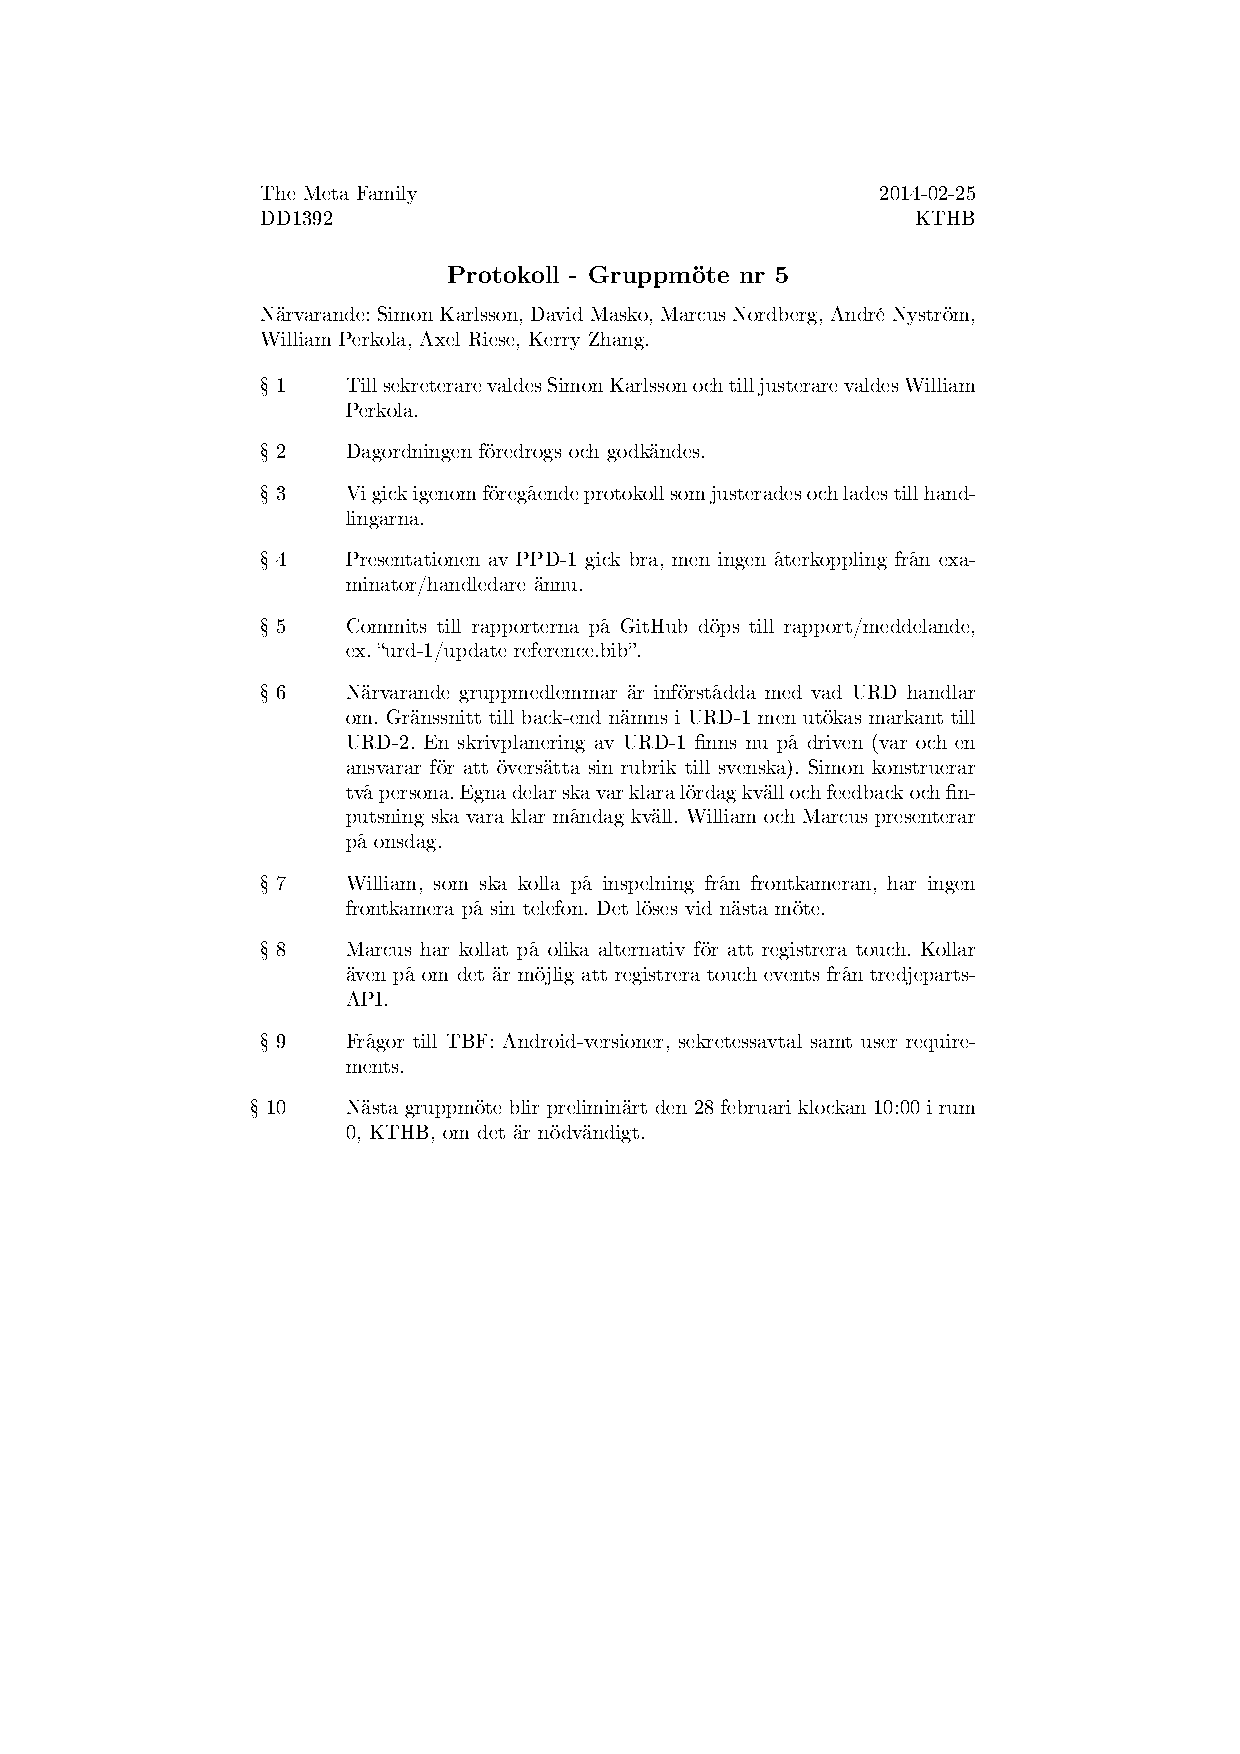
\includepdf{protokoll_2014-02-25}

\end{appendices}

\end{flushleft}
\end{document}
